\section{Interface de Utilizador} \label{sec:demonstracao}
Esta secção apresenta a interface de utilizador desenvolvida em Flutter, mostrando o fluxo principal e a materialização das funcionalidades do sistema.

\subsection{Ecrã Inicial} \label{subsec:ecra_inicial}
O ecrã inicial atua como o ponto central da aplicação, onde o utilizador pode monitorizar em tempo real o estado dos sensores ativos. 

Na versão \textit{Web}, presente na Figura \ref{subfig:web_intial_screen}, o espaço amplo permite a utilização de gráficos radiais (\textit{gauges}), dando um aspeto industrial adequado a painéis de controlo. Na versão \textit{Mobile} (Figura \ref{subfig:mobile_intial_screen}), a interface foi adaptada para cartões compactos, otimizando o espaço vertical do ecrã do telemóvel. Em termos de integração com o \textit{back-end}, assim que este ecrã é carregado, o \textit{front-end} inicia uma \textit{Subscription} GraphQL (via \textit{WebSockets}) para cada sensor listado, permitindo que qualquer nova medição processada pelo servidor seja imediatamente refletida na interface, sem necessidade de atualizar a página ou fazer pedidos repetitivos (\textit{polling}).

\begin{figure}[h]
	\centering
	\begin{subfigure}{0.65\linewidth}
		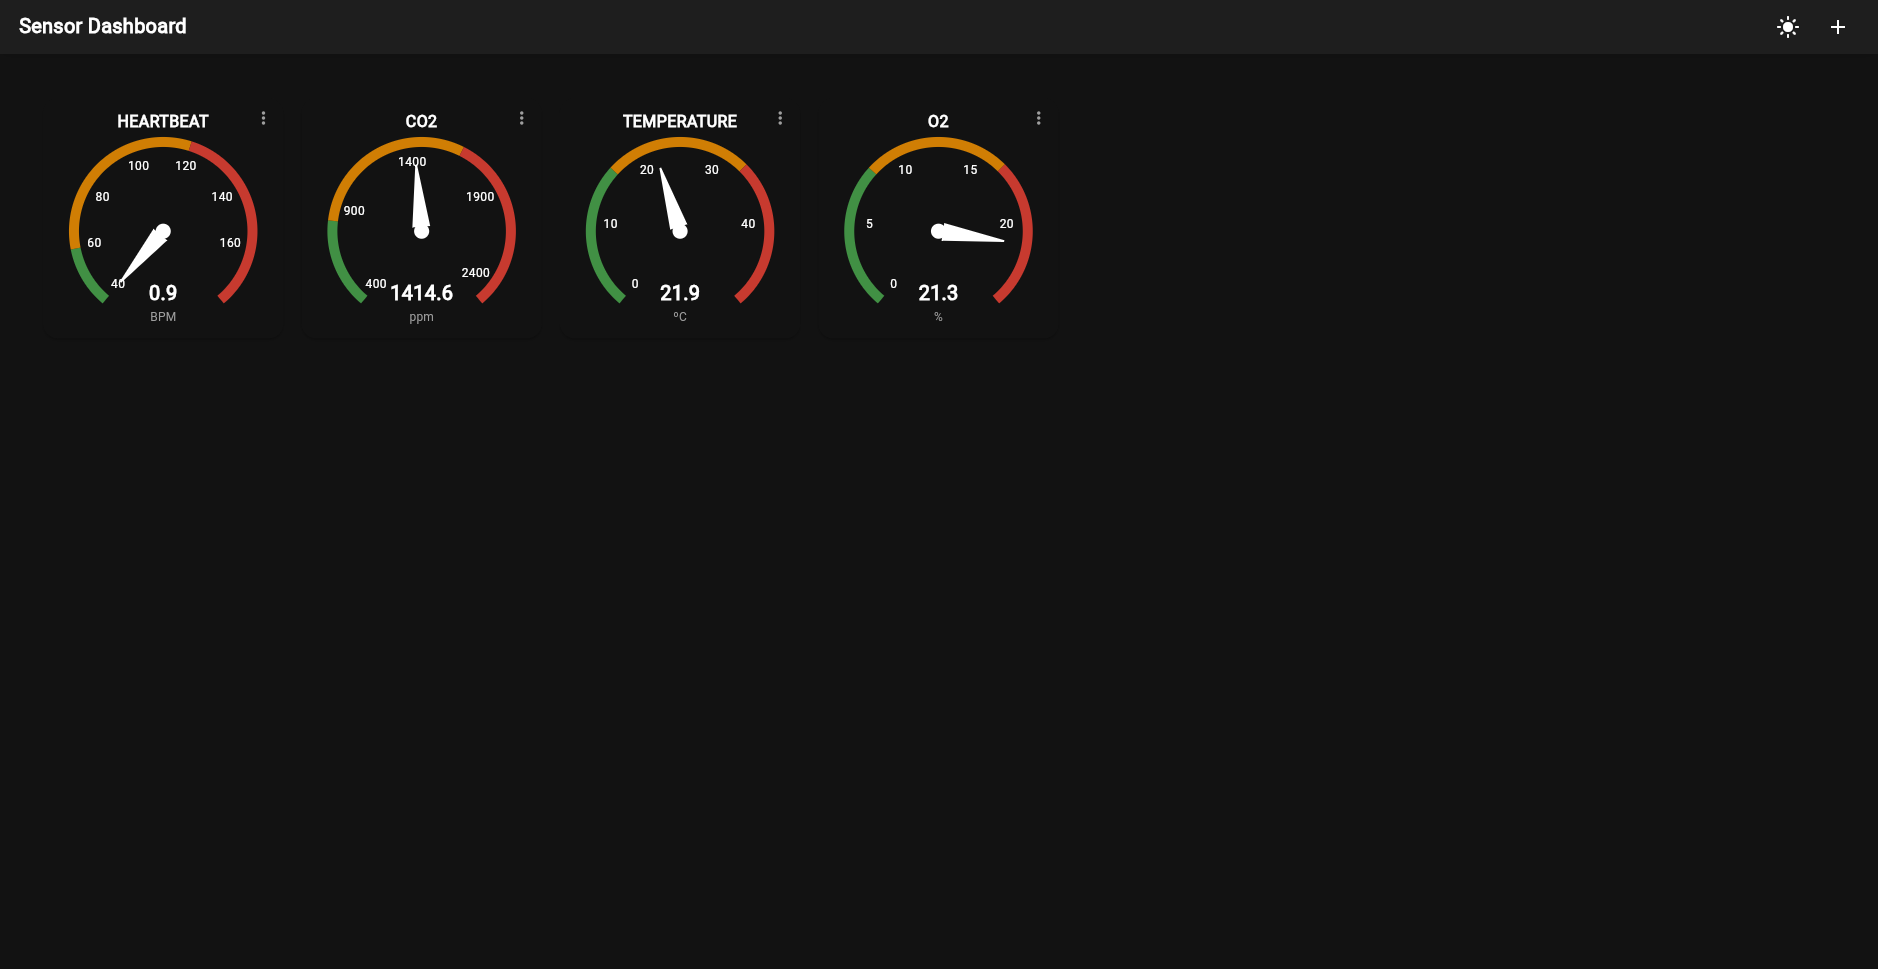
\includegraphics[width=\textwidth]{imagens/web_initial_screen.png}
		\caption{Interface Web}
		\label{subfig:web_intial_screen}
	\end{subfigure}
	\hfill
	\begin{subfigure}{0.30\linewidth}
		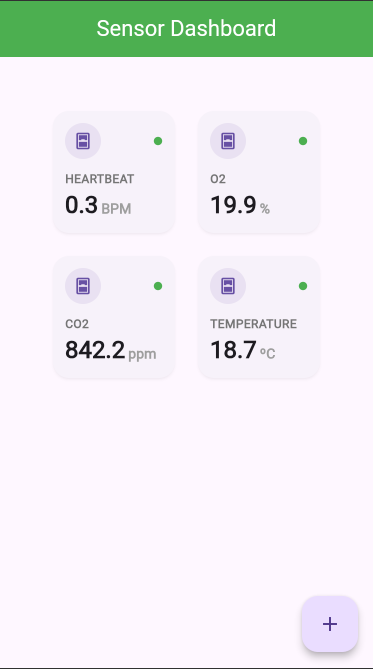
\includegraphics[width=\textwidth]{imagens/mobile_initial_screen.png}
		\caption{Interface Mobile}
		\label{subfig:mobile_intial_screen}
	\end{subfigure}
	
	\caption{Ecrã inicial com as medições dos sensores em tempo real.}
	\label{fig:initial_screen}
\end{figure}

\subsection{Ecrã para inserção de novos sensores}
Para adicionar novos sensores ao painel principal, o utilizador acede a um menu de seleção. Ao abrir essa interface, a aplicação executa uma \textit{Query} GraphQL ao \textit{back-end} para obter a lista atualizada de todos os nós e sensores registados na base de dados.

Devido às diferenças de navegação entre plataformas, na versão \textit{Mobile} (Figura \ref{subfig:mobile_add_sensor_screen}) esta funcionalidade é apresentada num ecrã dedicado, para haver uma área de toque maior. Por outro lado, na versão \textit{Web} (Figura \ref{subfig:web_add_sensor_screen}), a lista é apresentada sob a forma de uma janela sobreposta (\textit{Dialog}). Ao guardar a seleção, as escolhas são persistidas localmente no dispositivo e as respetivas \textit{subscriptions} de tempo real são ativadas no ecrã inicial.

\begin{figure}[h]
	\centering
	\begin{subfigure}{0.65\linewidth}
		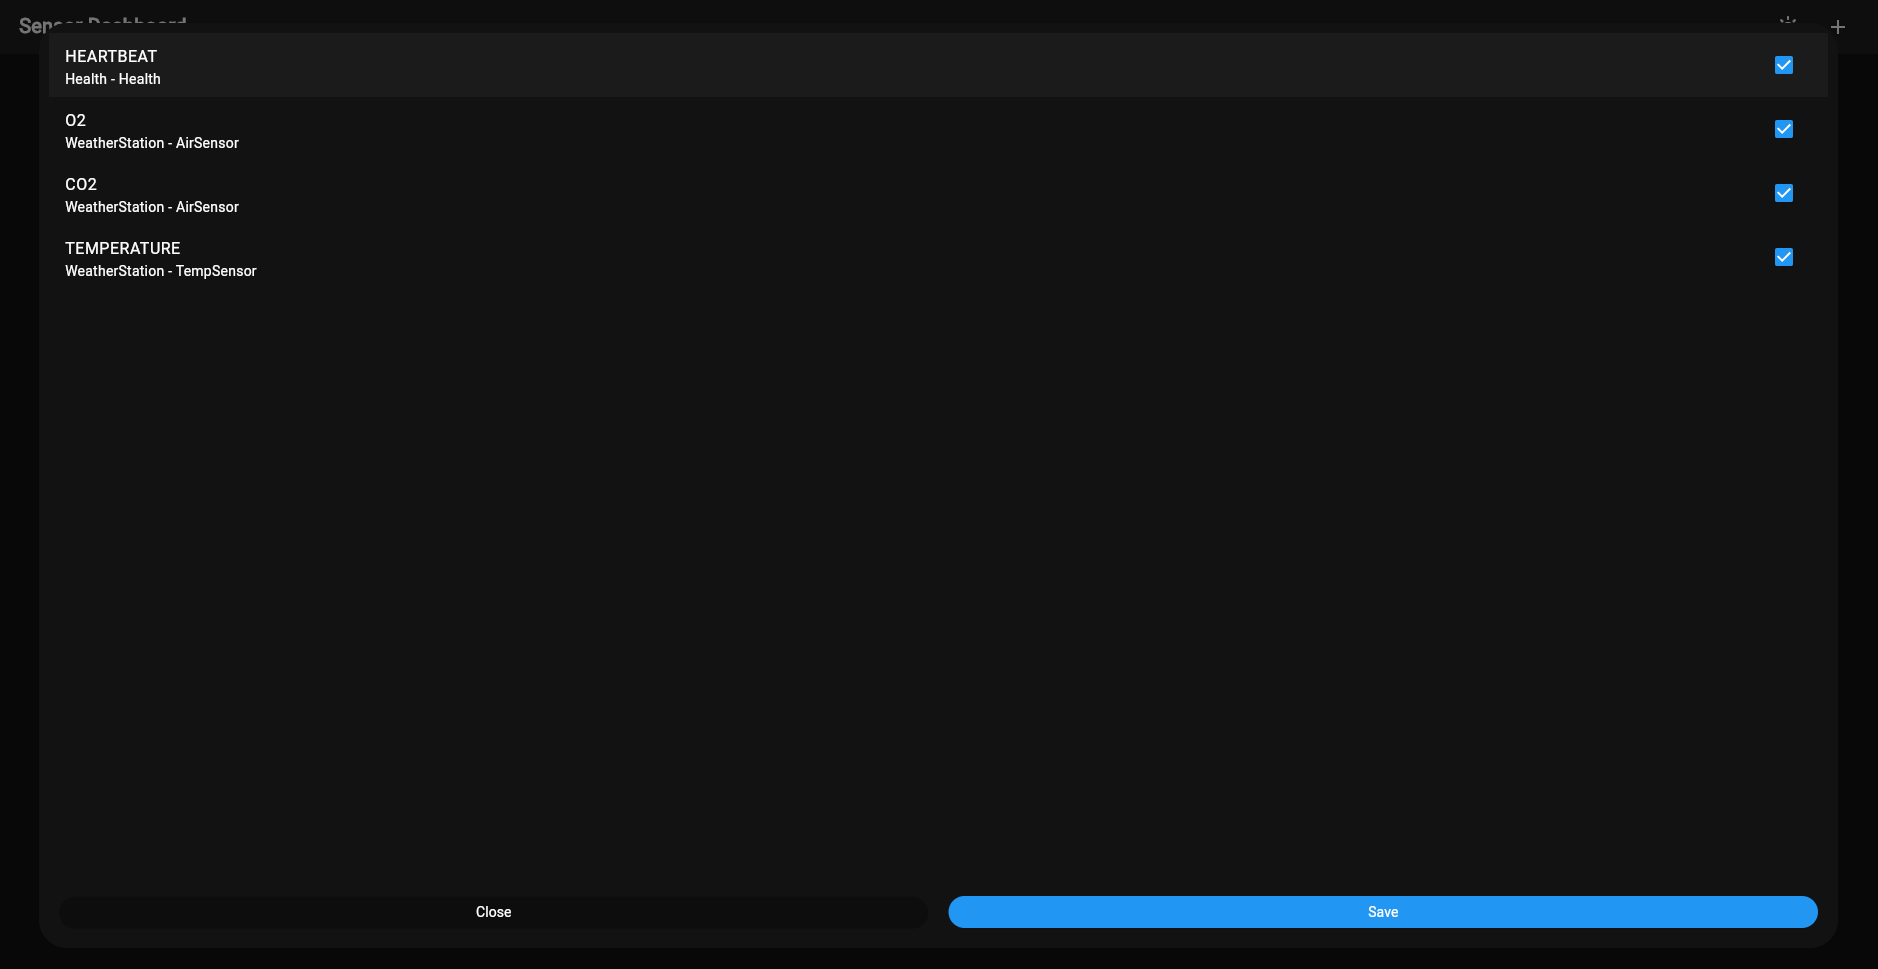
\includegraphics[width=\textwidth]{imagens/web_add_sensor_screen.png}
		\caption{Interface Web}
		\label{subfig:web_add_sensor_screen}
	\end{subfigure}
	\hfill
	\begin{subfigure}{0.30\linewidth}
		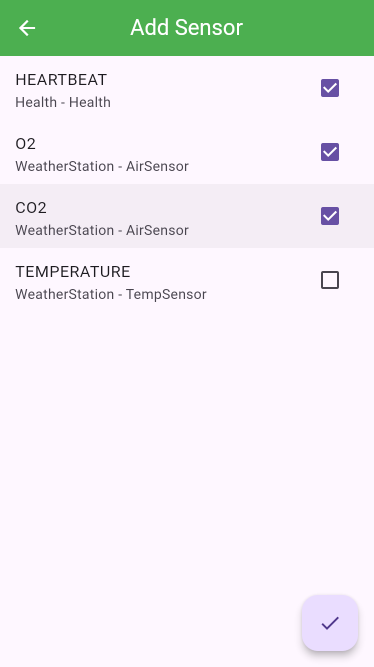
\includegraphics[width=\textwidth]{imagens/mobile_add_sensor_screen.png}
		\caption{Interface Mobile}
		\label{subfig:mobile_add_sensor_screen}
	\end{subfigure}
	
	\caption{Interface para adição e gestão de sensores no painel.}
	\label{fig:add_sensor_screen}
\end{figure}

\subsection{Gráfico histórico de medições}
A análise temporal dos dados é crucial para identificar tendências e anomalias. Ao selecionar um sensor específico, o utilizador tem acesso a um gráfico de linhas que ilustra o histórico recente de medições.

No gráfico, a integração com o servidor ocorre em duas fases simultâneas: primeiro, uma \textit{Query} GraphQL é realizada para carregar o histórico de dados guardados na base de dados, de modo a desenhar a linha inicial; de seguida, os dados provenientes da \textit{subscription} em tempo real são injetados diretamente no gráfico, fazendo com que a linha avance dinamicamente. Na versão \textit{Web} (Figura \ref{subfig:web_data_temporal_chart}), este gráfico é exibido através de um painel lateral (\textit{Side Panel}). Na aplicação \textit{Mobile} (Figura \ref{subfig:mobile_data_temporal_chart}), devido às limitações físicas do ecrã, o gráfico é exibido num novo ecrã.

\begin{figure}[h]
	\centering
	\begin{subfigure}{0.65\linewidth}
		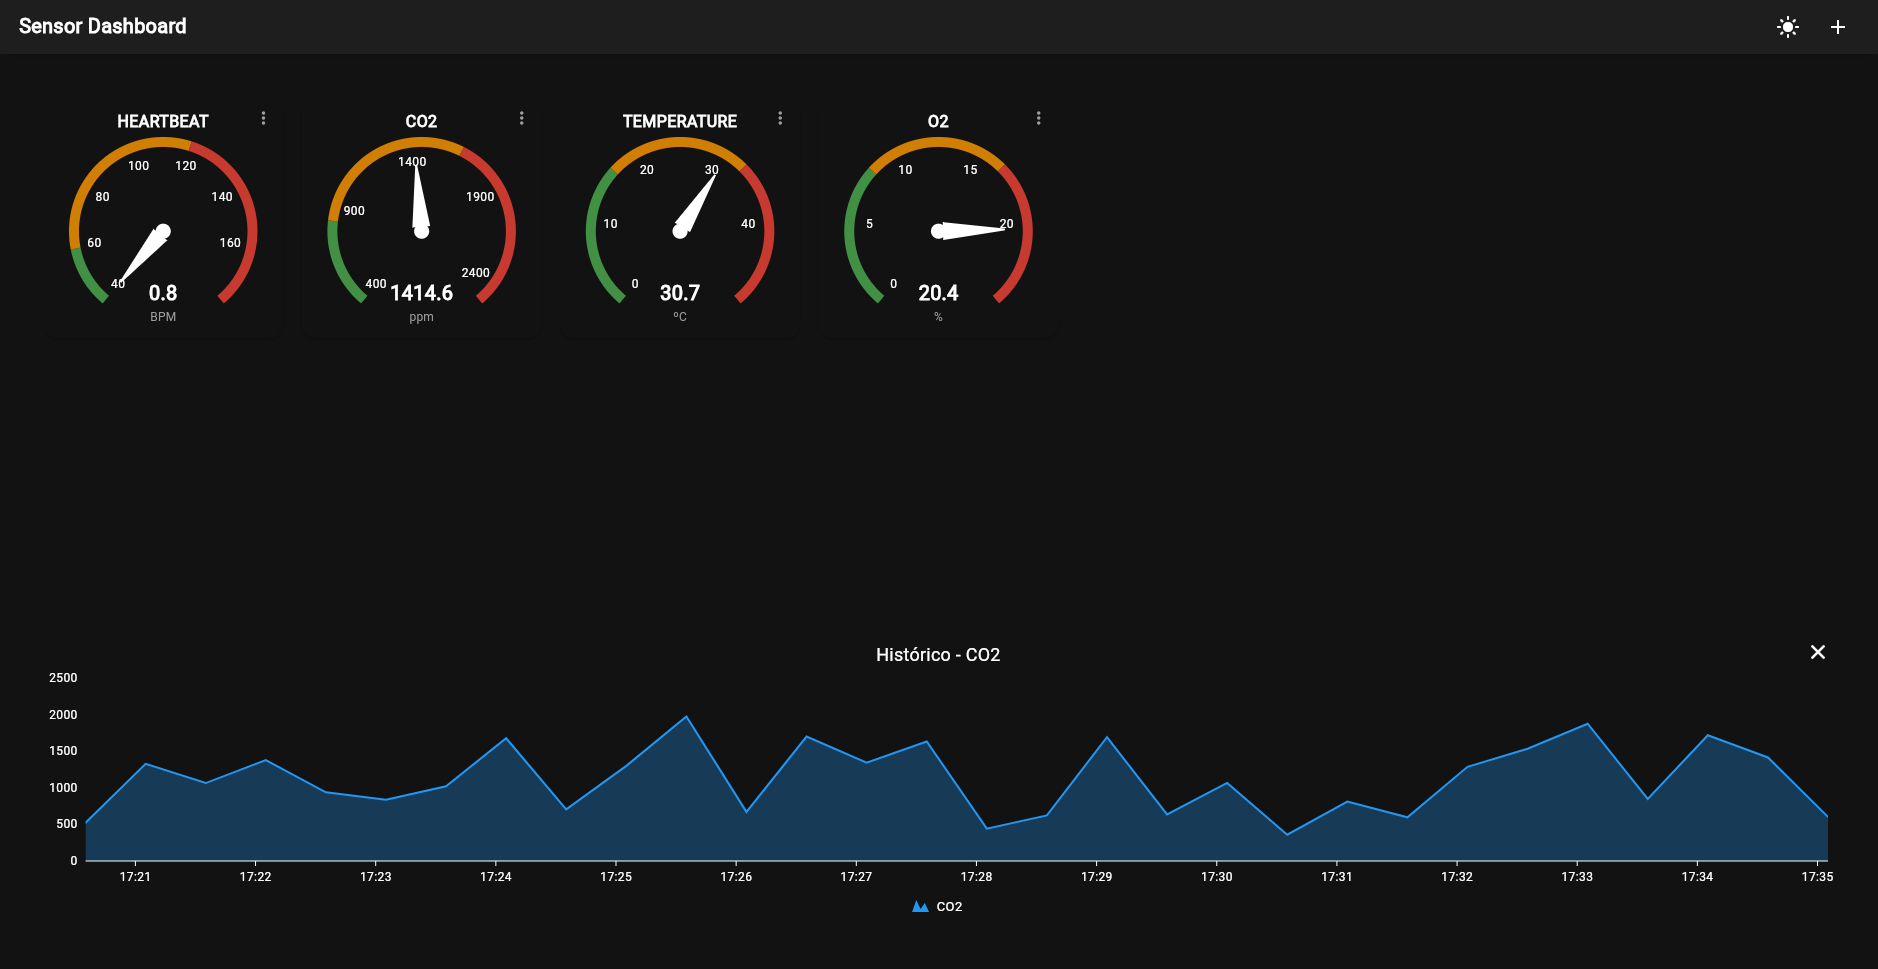
\includegraphics[width=\textwidth]{imagens/web_data_temporal_chart.png}
		\caption{Interface Web}
		\label{subfig:web_data_temporal_chart}
	\end{subfigure}
	\hfill
	\begin{subfigure}{0.30\linewidth}
		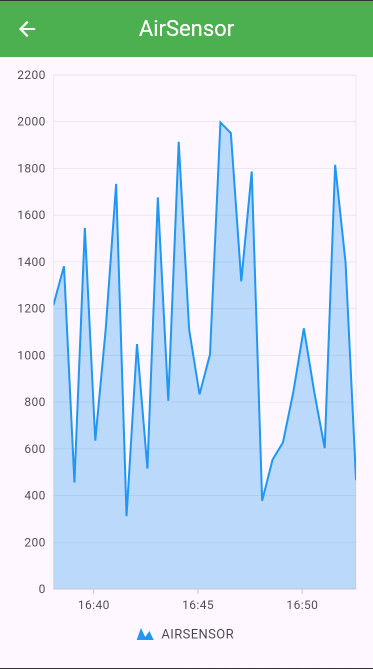
\includegraphics[width=\textwidth]{imagens/mobile_data_temporal_chart.png}
		\caption{Interface Mobile}
		\label{subfig:mobile_data_temporal_chart}
	\end{subfigure}
	
	\caption{Gráfico com o histórico temporal de medições de um sensor selecionado.}
	\label{fig:data_temporal_chart}
\end{figure}

\subsection{Alterar mínimos e máximos}

Como referido na Secção \ref{subsec:ecra_inicial}, o \textit{dashboard} \textit{Web} utiliza gráficos radiais (\textit{Gauges}), que necessitam de limites pré-definidos para contextualizar adequadamente se as medições estão dentro de um intervalo admissível.

Embora os sensores recebam valores genéricos ao serem adicionados, o utilizador pode ajustá-los através de uma janela sobreposta (\textit{Dialog}), acessível no canto superior direito de cada mostrador (Figura \ref{fig:web_change_min_max}). Esta parametrização ajusta dinamicamente a escala do gráfico, permitindo focar a monitorização num intervalo de valores mais exato.

Adicionalmente, este painel permite a remoção rápida do sensor. Todas as alterações efetuadas são guardadas de forma persistente através das preferências locais (\textit{SharedPreferences}), assegurando que as configurações visuais não se perdem ao reiniciar a aplicação.

\begin{figure}[h]
	\centering
	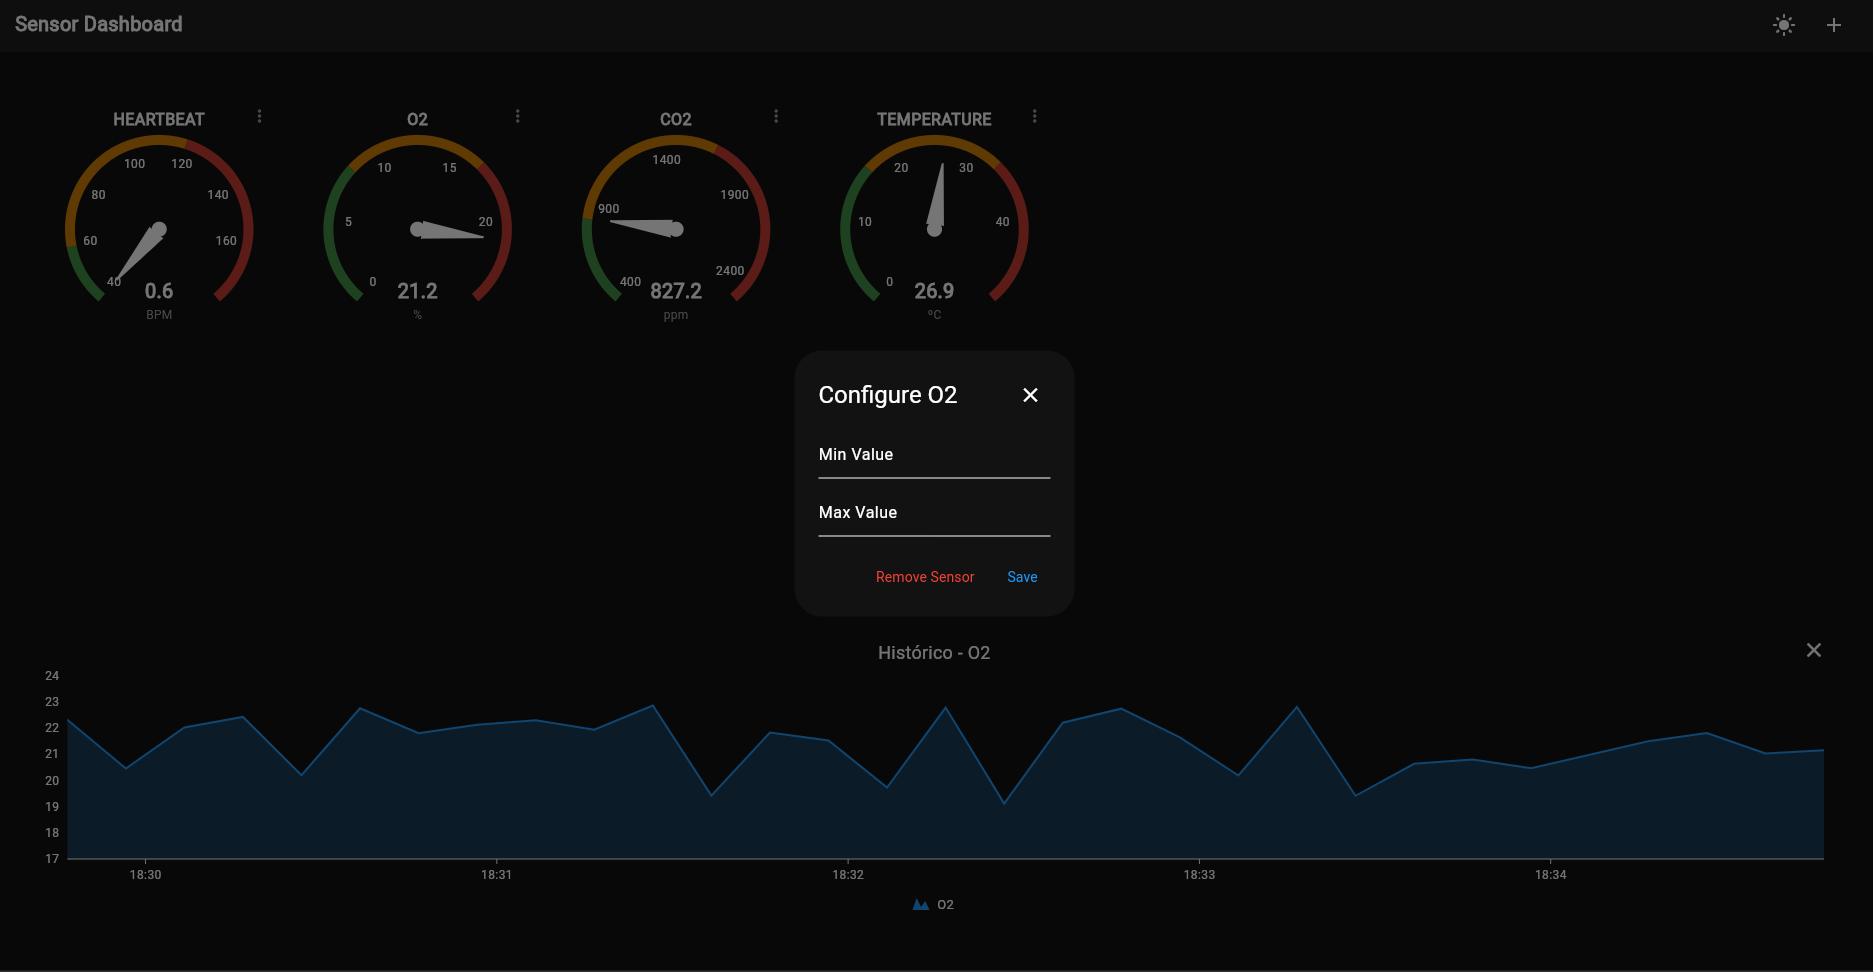
\includegraphics[width=0.7\linewidth]{imagens/web_change_min_max}
	\caption{Dialog para edição dos limites do mostrador e remoção do sensor.}
	\label{fig:web_change_min_max}
\end{figure}
